\chapter{Literature Review}
\label{chap:lit-review}

This chapter provides a literature review of relevant past research efforts 
giving context to this dissertation. 
I begin with an overview of the \gls{FHR} concept, then detail one specific 
\gls{FHR} design: the \gls{AHTR}. 
I describe previous efforts and technical challenges of modeling the \gls{AHTR} design, 
and how these efforts led to the \gls{OECD} \gls{NEA}'s \gls{FHR} benchmark initiation.
Next, I outline additive manufacturing's history and describe the current 
research on using additive manufacturing for nuclear reactor component fabrication. 
I review previous nuclear reactor design optimization efforts and describe how 
additive manufacturing of nuclear reactor components enables optimization for 
less constrained reactor geometries. 
I describe optimization methods that can be leveraged to find optimal reactor 
designs in the expanded design space.
Finally, I give a background of the evolutionary algorithms and detail a specific 
evolutionary algorithm: the genetic algorithm and how it works to conduct global 
optimization robustly.

\section{Fluoride-Salt-Cooled High-Temperature Reactor System}
\label{sec:fhr}
To ensure continued global use and expansion of nuclear energy technology, in 
2001, the \gls{OECD} and nuclear energy experts initiated the \gls{GIF} 
\cite{gen_iv_international_forum_technology_2014}.
The \gls{GIF} aims to enhance the role of nuclear energy in our global energy 
ecosystem by coordinating global research and development to test the 
feasibility and performance of Generation IV nuclear reactor systems to enable 
their industrial deployment by 2030 \cite{gen_iv_international_forum_technology_2014}.
The \gls{GIF} selected six Generation IV systems for further research and 
development based on target goals in four areas: sustainability, 
economics, safety and reliability, and proliferation resistance and physical 
protection \cite{gen_iv_international_forum_technology_2014}. 
Table \ref{tab:goals-gen4} summarizes the goals in each area. 
\begin{table}[htb!]
    \centering
    \onehalfspacing
    \caption{Goals of Generation IV Nuclear Systems \cite{gen_iv_international_forum_technology_2014,
    gen_iv_international_forum_technology_2014}}
	\label{tab:goals-gen4}
    \footnotesize
    \begin{tabular}{l|l}
    \hline
                               \textbf{Area} & \textbf{Goals} \\ \hline
    Sustainability   & - Have a positive impact on the environment through the displacement of \\
    & polluting energy and transportation sources by nuclear electricity generation \\
    & and nuclear-produced hydrogen \\ 
    & - Promote long-term availability of nuclear fuel \\
    & - Minimize volume, lifetime, and toxicity of nuclear waste \\ \hline
    Economics & - Have a life cycle and energy production cost advantage over other energy \\
    & sources \\ 
    & - Reduce economic risk to nuclear projects by developing plants using \\
    & innovative fabrication and construction techniques \\ \hline
    Safety and Reliability   & - Increase the use of robust designs and inherent and transparent safety\\
    & features that non-experts can understand \\ 
    & - Enhance public confidence in the safety of nuclear energy \\\hline
    Proliferation Resistance & - Provide continued effective proliferation resistance of nuclear energy \\
    and Physical Protection & systems through improved design features and other measures \\ 
    & - Increase the robustness of new facilities \\ \hline
    \end{tabular}
\end{table}
The systems selected are \glspl{GFR}, \glspl{LFR}, \glspl{MSR}, \glspl{SFR}, \glspl{SCWR}, 
and \glspl{VHTR} \cite{gen_iv_international_forum_technology_2014}. 
The \acrfull{FHR} concept introduced in 2003 uses a low-pressure liquid fluoride-salt 
coolant and high-temperature coated-particle \gls{TRISO} fuel, combining 
the best aspects of the \gls{MSR} and \gls{VHTR} systems respectively
\cite{forsberg_molten-salt-cooled_2003,facilitators_fluoride-salt-cooled_2013}.

\gls{MSR} systems produce fission power in a circulating molten salt fuel 
mixture. 
Molten salt reactor coolants introduce inherent safety due to the 
low system vapor pressure and the salts' high boiling temperature and 
volumetric heat capacity \cite{ho_molten_2013}.
Fluoride salt used in \glspl{FHR} is Li$_2$BeF$_4$, also known as \gls{FLiBe}, 
which remains liquid without pressurization up to 1400 $^{\circ}$C and has a greater 
heat capacity than water \cite{ho_molten_2013,forsberg_fluoride-salt-cooled_2012}.
Researchers recommend molten fluoride salts because they have high uranium 
solubility, chemical stability, low vapor pressure at high temperatures, 
good heat transfer properties, radiation damage resistance, and are inert 
to common structural materials \cite{rosenthal_molten-salt_1970}. 
\gls{VHTR} systems use a once-through uranium cycle and leverage 
high outlet temperatures for high-temperature heat applications, such as 
hydrogen production. 
Graphite-moderated and helium-cooled \glspl{VHTR} use \gls{TRISO} fuel
which withstands high burnup and temperature, enabling higher operating 
temperatures \cite{gen_iv_international_forum_technology_2014}.  
Higher operating temperatures advantages include increased power 
conversion efficiency, reduced waste heat generation, and co-generation and 
process heat capabilities \cite{scarlat_design_2014}.
However, the \glspl{VHTR} system's helium coolant is at 100 atm requiring a 
thick concrete vessel. 

By combining \gls{FLiBe} coolant from \gls{MSR} technology and 
\gls{TRISO} fuel from \gls{VHTR} technology, the \gls{FHR} benefits from 
low operating pressure and large thermal margin enabled by the molten fluoride
salt coolant and the thermal resilience of \gls{TRISO} particle fuel. 
The low vapor pressure in molten fluoride salts ensures reduced stress on the system
and increased safety compared to the \gls{VHTR}'s high operating pressure. 
\gls{TRISO} solid fuel cladding in the \gls{FHR} system adds an extra barrier 
to fission product release compared to \glspl{MSR} with liquid fuel 
\cite{ho_molten_2013}.

Several types of \gls{FHR} conceptual designs exist worldwide: the \gls{PBFHR} 
developed at \gls{UCB} with circulating pebble-fuel 
\cite{scarlat_current_2014,krumwiede_three-dimensional_2013}, the \gls{SF-TMSR} 
developed at the \gls{SINAP} with static pebble-fuel \cite{liu_preliminary_2016}, 
the large central-station \gls{AHTR} at \gls{ORNL} \cite{holcomb_core_2011, varma_ahtr_2012}, 
and the \gls{SmAHTR} at ORNL \cite{greene_pre-conceptual_2010} with static, 
plate fuel. 

\subsection{\acrlong{AHTR} Design}
This dissertation focuses on the prismatic \gls{FHR} design with hexagonal fuel 
assemblies consisting of \gls{TRISO} fuel particles embedded in planks, i.e., 
the \gls{AHTR} design developed by ORNL. 
The \gls{AHTR} has 3400 MWt thermal power and 1400 MW electric power with
inlet/outlet temperatures of 650/700$^{\circ}$C \cite{varma_ahtr_2012}.  
Figure \ref{fig:ahtr} shows the prismatic AHTR's fuel assembly and core 
configuration.  
\begin{figure}[htb!]
    \centering
    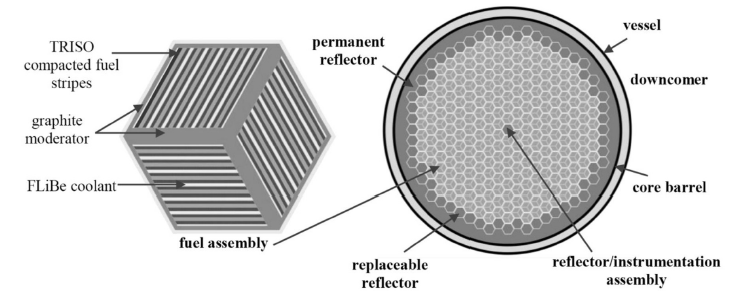
\includegraphics[width=\linewidth]{ahtr.png} 
    \caption{\acrlong{AHTR} fuel assembly (left) and core configuration (right) 
    reproduced from \cite{ramey_monte_2018}.}
    \label{fig:ahtr}
\end{figure}
Each hexagonal fuel assembly features plate-type fuel consisting of eighteen 
planks arranged in three diamond-shaped sectors, with a central Y-shaped 
structure and external channel (wrapper).
The fuel planks contain an isostatically pressed carbon with fuel stripes 
on each plank's outer side.
Within each fuel stripe is a graphite matrix filled with \gls{TRISO} particles. 
The core consists of 252 assemblies radially surrounded by reflectors
\cite{ramey_monte_2018}. 
Chapter \ref{chap:fhr-benchmark} details the specifications of the AHTR geometry
modeled in this dissertation.

\subsection{Previous AHTR modeling efforts and challenges} 
\label{sec:previous_ahtr}
Most state-of-the-art reactor simulation tools today have been designed for 
\gls{LWR} analysis.
The \gls{AHTR} core design differs significantly from the currently operating \gls{LWR} 
cores.  
These differences lead to modeling challenges with the current tools, highlighting
the need to verify and validate current simulation tools for \gls{AHTR} physics 
\cite{ramey_monte_2018}. 
Verification and validation of \gls{AHTR} neutronics and thermal-hydraulics 
simulation capabilities support the \gls{AHTR} design's licensure and the
eventual goal of \gls{AHTR} deployment 
\cite{rahnema_phenomena_2019,rahnema_current_2015}.
This section outlines the previous efforts to model and validate 
the \gls{AHTR}'s neutronics and thermal-hydraulics. 

\subsubsection{AHTR Neutronics Modeling}
Several neutronics studies conducted to support the current iteration of the \gls{AHTR} 
design have illuminated the design's technical challenges 
\cite{ramey_monte_2018,holcomb_fluoride_2013,greene_pre-conceptual_2010}. 
\gls{Georgia Tech} led an Integrated Research Project to understand \gls{AHTR} 
material and modeling challenges \cite{zhang_integrated_2019}. 
During the research project, a panel of subject matter experts 
generated a \gls{PIRT}.
The \gls{PIRT} identifies \gls{AHTR} areas that need additional research to better 
understand important phenomena for adequate future modeling
\cite{rahnema_phenomena_2019}. 
Table \ref{tab:phenomena} lists the phenomena identified as requiring further 
research. 
\begin{table}[htb!]
    \centering
    \onehalfspacing
    \caption{\acrlong{PIRT} identified \acrlong{AHTR} physical phenomena requiring 
    further research \cite{rahnema_phenomena_2019}.}
	\label{tab:phenomena}
    \footnotesize
    \begin{tabular}{l|l}
    \hline
    \textbf{Category} & \textbf{Phenomena} \\ \hline
    Fundamental cross section data & - Moderation in FliBe \\
    & - Thermalization in FliBe \\
    & - Absorption in FliBe \\
    & - Thermalization in carbon \\
    & - Absorption in carbon \\ \hline
    Material Composition & - Fuel particle distribution \\ \hline
    Computational Methodology & - Solution Convergence \\ 
    & - Granularity of depletion regions \\
    & - Multiple heterogeneity treatment for generating multigroup \\ 
    & cross sections \\
    & - Selection of multigroup structure \\
    & - Boundary conditions for multigroup cross section generation \\ \hline 
    General Depletion & - Spectral history \\ \hline 
    \end{tabular}
\end{table}

The \emph{triple heterogeneous} \gls{AHTR} fuel, comprised of \gls{TRISO} 
particles embedded in strategically arranged plates, presents simulation 
challenges. 
Researchers must obtain detailed reference power distributions with individual 
\gls{TRISO} particle fidelity to understand nuances in the physics, such 
as self-shielding.
Deterministic codes that use multigroup cross sections and traditional 
homogenization methods \cite{ramey_monte_2018}, insufficiently capture the 
\glspl{AHTR} physics due to these multiple heterogeneities 
\cite{ramey_monte_2018}. 
In the \gls{AHTR}, single and multiple slab homogenization decreased total 
neutron transport simulation time by an order of 10; however, the homogenization 
introduced a nontrivial $k_{eff}$ error of $\sim$3\% 
\cite{ramey_monte_2018, cisneros_neutronics_2013}.
To determine the feasibility and safety of the \gls{AHTR} design, researchers 
must calculate core physics parameters to an acceptable uncertainty. 
With Monte Carlo neutron transport, increasing neutron histories reduces statistical 
uncertainty but increases computational cost typically, requiring
supercomputers to run the simulations.

This \gls{AHTR} presents another technical challenge: the uncertainty of 
graphite moderator material properties: densities, temperatures, and thermal 
scattering data.
Also, the thermal scattering data ($S(\alpha,\beta)$ matrices) for 
the bound nuclei in \gls{FLiBe} salts are lacking \cite{ramey_monte_2018}. 
Mei et al. \cite{mei_investigation_2013} and Zhu et al. \cite{zhu_thermal_2017} 
examined the thermal scattering behavior of solid and liquid \gls{FLiBe}.
They concluded that the bound and free atom cross section of \gls{FLiBe} are 
identical above 0.1eV and diverge below 0.01eV, which means that the use or 
absence of thermal scattering data will impact the accuracy of the results 
\cite{ramey_monte_2018}. 

\subsubsection{AHTR Multiphysics Modeling}
In a past effort toward \gls{AHTR} multiphysics modeling, Gentry et al. 
\cite{gentry_development_2016} developed an adapted lattice physics-to-core 
simulator two-step procedure with Serpent \cite{leppanen_serpent_2014} 
and \gls{NESTLE} \cite{turinsky_nestle_1994} for the \gls{AHTR} design. 
The adapted lattice physics-to-core simulator two-step procedure proved to be 
successful for \glspl{LWR}. A 2-D transport lattice calculation generates the 
\gls{LWR}'s group assembly homogenized group constants, and then core 
analysis is performed by 3-D nodal simulation 
\cite{koebke_new_1980,gentry_development_2016}.
\gls{NESTLE}'s thermal-hydraulics utilizes a \gls{HEM} model for two-phase 
flow, and it solves the few-group neutron diffusion equation utilizing the
\gls{NEM} for cartesian and hexagonal reactor geometries.  
Gentry et al. concluded that the method required accuracy improvements 
by improving the reflector model and further optimizing the coarse energy group 
structure.
Lin \cite{lin_thermal_2020} used RELAP5, a system-level code, to perform 
\gls{AHTR} thermal hydraulics transient simulations to investigate the 
capability of the passive heat removal system. 
In the RELAP5 model, Lin separated the \gls{AHTR}'s 252 assemblies into 
four concentric rings with uniform power distribution per ring. 
Lin also gives higher fidelity in the primary and \gls{DRACS} system loops. 
Lin utilized RELAP5 in transient scenarios to determine 
the temperature at various locations in the system loop by assuming a power 
value for fuel assemblies in each ring \cite{lin_thermal_2020}. 
However, this method is not ideal for transient scenarios with tightly coupled 
neutronics and thermal-hydraulics. 

\subsection{FHR Benchmark}
The previous section highlights the singular efforts to model 
different aspects of the \gls{AHTR}'s neutronics and thermal hydraulics, with
each author describing their modeling difficulties. 
However, there lacked a robust and methodical method for evaluating the 
simulation software and comparing the \gls{AHTR} modeling results generated by 
individual researchers.

To gain a comprehensive view of the \gls{AHTR}'s modeling challenges and 
cross-verify available \gls{AHTR} modeling tools, in 2019, the 
\gls{OECD}-\gls{NEA} initiated the \gls{FHR} benchmarking exercise 
of the \gls{AHTR} design \cite{petrovic_benchmark_2021}.
Several organizations participate in the benchmark with various Monte Carlo
and Deterministic neutronics software, such as Serpent \cite{leppanen_serpent_2014}, 
OpenMC \cite{romano_openmc_2013}, and WIMS \cite{lindley_current_2017}. 

The benchmark has three phases: a single fuel assembly simulation 
without burnup (Phase I), full core depletion (Phase II), and multiphysics 
feedback (Phase III). 
The benchmark aims to identify the latest codes' applicability, accuracy, 
and practicality to assess the current state-of-the-art FHR simulation 
and modeling \cite{petrovic_preliminary_2021}. 
The benchmark also enables the cross-verification of software and methods 
for the challenging \gls{AHTR} geometry, which is especially useful since 
applicable reactor physics experiments for code validation are scarce 
\cite{petrovic_fhrahtr_2019,petrovic_preliminary_2021}. 
Chapter \ref{chap:fhr-benchmark} will provide a detailed description of the 
benchmark's phases and results.

\subsection{Modeling Software}
\label{sec:lit-review-modeling-software}
In this dissertation, I use OpenMC \cite{romano_openmc:_2015} to model \gls{AHTR}'s 
neutronics and Moltres \cite{lindsay_introduction_2018} to model the \gls{AHTR}'s 
temperature. 
In the following subsections, I will describe the capabilities of each software 
and motivate their use for my dissertation. 

\subsubsection{OpenMC}
OpenMC \cite{romano_openmc:_2015} is a continuous-energy Monte Carlo neutron transport 
open-source code hosted on Github.
It was created in 2011 at \gls{MIT} as part of an effort to develop scalable parallel 
Monte Carlo neutron transport algorithms for future exascale supercomputers 
\cite{romano_openmc:_2015}, and is currently supported by resources from \gls{ANL}. 
OpenMC runs in parallel using \gls{MPI} and OpenMP. 
Many components of OpenMC have been validated and verified with experimental data 
and other well-established neutron transport codes through benchmarks 
\cite{romano_openmc:_2015}. 

OpenMC is capable of performing fixed source and k-eigenvalue calculations. 
This dissertation uses OpenMC's k-eigenvalue calculations for \gls{AHTR} neutronics 
modeling.
OpenMC represents neutron interaction with various nuclei in the ACE format 
\cite{x-5_monte_carlo_team_mcnp_2003}.
The NJOY nuclear data processing system \cite{macfarlane_njoy_2017} converts the 
raw ENDF/B data into linearly-interpolable ACE-format data, enabling the nuclear 
data libraries to provide continuous energy cross section data at discrete temperatures.
OpenMC models use constructive solid geometry representation; they provide standard 
geometric surfaces (e.g. planes, cylinders) for defining reactor geometries.  
This dissertation uses v0.12.2 of OpenMC with the ENDF VII.1 nuclear data library
\cite{chadwick_endf/b-vii.1_2011}. 
% Based on results of other benchmarks, why did you choose this software? 

\subsubsection{Moltres}
Moltres is an open-source tool designed to simulate \glspl{MSR} using 
deterministic neutronics and thermal-hydraulics implemented as an application 
atop the \gls{MOOSE} finite-element framework.  
Moltres solves arbitrary group neutron diffusion, temperature, and precursor 
governing equations on a single mesh and can be deployed on an arbitrary number 
of processing units \cite{lindsay_introduction_2018, park_advancement_2020}.
To perform neutronics calculations, Moltres requires group constant data from 
high-fidelity neutronics software such as OpenMC \cite{romano_openmc:_2015} or 
Serpent 2 \cite{leppanen_serpent_2014}. 
Users run a Python script in Moltres' Github repository, which automatically reads
user-provided OpenMC/Serpent 2 output files and creates Moltres-compatible JSON 
containing all required group constant data.

Moltres solves for the neutron fluxes governed by the multigroup neutron diffusion 
equations:
\begin{align}
    \label{eq:moltres-diffusion-equation}
    \frac{1}{v_g} \frac{\partial \phi_g}{\partial t} &= \nabla \cdot D_g
    \nabla \phi_g - \Sigma^r_g \phi_g +
    \sum^G_{g' \neq g} \Sigma^s_{g' \rightarrow g} \phi_{g'} + \chi^p_g
    \sum^G_{g'=1} (1-\beta) \nu \Sigma^f_{g'} \phi_{g'} + \chi^d_g \sum^I_i
    \lambda_i C_i \\
    \intertext{where}
    v_g &= \text{ average speed of neutrons in group $g$ [$cm \cdot s^{-1}$],} \nonumber \\
    \phi_g &= \text{ neutron flux in group $g$ [$cm^{-2} \cdot s^{-1}$],}\nonumber \\
    t &= \text{ time $[s]$,} \nonumber \\
    D_g &= \text{ diffusion coefficient of neutrons in group $g$ [$cm^{-2} \cdot s^{-1}$],} \nonumber \\
    \Sigma^r_g &= \text{ macroscopic cross section for removal of neutrons from group $g$ [$cm^{-1}$],} \nonumber \\
    \Sigma^s_{g' \rightarrow g} &= \text{ macroscopic cross section of scattering from groups $g'$ to $g$ [$cm^{-1}$],} \nonumber \\
    \chi^p_g &= \text{ prompt fission spectrum for neutrons in group $g$ [-],} \nonumber \\
    G &= \text{ total number of discrete neutron groups [-],} \nonumber \\
    \nu &= \text{ average number of neutrons produced per fission [-],} \nonumber \\
    \Sigma^f_{g} &= \text{ macroscopic fission cross section for neutron in group $g$ [$cm^{-1}$],} \nonumber \\
    \chi^d_g &= \text{ delayed fission spectrum for neutrons in group $g$ [-],} \nonumber \\
    I &= \text{ total number of delayed neutron precursor groups [-],} \nonumber \\
    \beta &= \text{ total delayed neutron fraction [-].} \nonumber
\end{align} 

Moltres' governing temperature equation is an advection-diffusion
equation with a fission heat source term $Q_f$: 
\begin{align}
    \label{eq:moltres-temp}
    \rho c_{p} \frac{\partial T}{\partial t} &= - \rho c_p \vec{u}
    \cdot \nabla T + \nabla \cdot \left(k \nabla T \right) + Q_f
    \intertext{and}
    Q_f &= \sum^G_{g=1} \epsilon_g \Sigma_g^f \phi_g
    \intertext{where}
    \rho =& \text{ density of the molten salt [$g \cdot cm^{-3}$],} \nonumber \\
    c_p =& \text{ specific heat capacity of molten salt [$J \cdot g^{-1} \cdot K^{-1}$],} \nonumber \\
    T =& \text{ temperature of molten salt [K],} \nonumber \\
    k =& \text{ thermal conductivity of molten salt [$W \cdot cm^{-1} \cdot K^{-1}$],} \nonumber \\
    Q_f =& \text{ fission heat source [$W cm^{-3}$],} \nonumber \\
    \epsilon_g =& \text{ average fission energy released by neutrons in group $g$ [J].} \nonumber \\
    \Sigma^f_{g} &= \text{ macroscopic fission cross section for neutron in group $g$ [$cm^{-1}$],} \nonumber \\
    \phi_g &= \text{ neutron flux in group $g$ [$cm^{-2} \cdot s^{-1}$],}\nonumber 
\end{align} 
% todo: how do neutronics and TH couple in moltres? why is it a good choice for this 
% work? what has been done previously with it? 
% Todo: ask sm 

\section{Additive Manufacturing}
Additive manufacturing is the formal term for what is popularly known as `3D printing' 
\cite{gibson_additive_2014}. 
The basic principle of additive manufacturing is that a model is initially generated using a
\gls{3D CAD} system and then fabricated directly without process planning. 
As the name implies, additive manufacturing adds material in layers. 
Each layer is a thin cross section of a \gls{3D CAD}-designed part, as opposed 
to traditional machining, which subtracts material instead 
\cite{standard_standard_2012}. 
All commercialized additive manufacturing machines to date use a layer-based 
approach.
The methods differ in the following ways: materials, layer creation method, and 
how the layers are bonded \cite{gibson_additive_2014}.
These major differences will determine the: accuracy of the 
final part, material and mechanical properties, time required to manufacture 
the part, need for post-processing, size of additive manufacturing machine, and overall 
cost of the machine and the process \cite{gibson_additive_2014}. 
Initially, industries only utilized additive manufacturing for manufacturing 
prototypes. 
However, with improvements in material properties, accuracy, and overall 
quality of additive manufacturing output, the applications for additive 
manufacturing have advanced. 
Industries have begun 3D printing parts for direct assembly purposes, 
such as air-cooling ducts for aircraft, hearing aids, and prosthesis
\cite{uriondo_present_2015}.  

Additive manufacturing has progressed rapidly in the last 30 years, from rapid 
design prototyping with polymers in the automotive industry to scale production 
of metal components.  
Examples include Boeing using additive manufacturing to reduce the 979 
Dreamliner's weight \cite{noauthor_printed_2017} and General Electric using 
additive manufacturing to produce fuel injection nozzles 
\cite{noauthor_transformation_2018}. 
The most common metal additive manufacturing technologies, \gls{SLM}, \gls{EBM}, 
\gls{L-DED}, and binder jetting, are not currently used to manufacture nuclear 
power plant parts. 

The U.S. \gls{DOE}, National Laboratories, and \gls{EPRI} support research and 
development efforts toward deploying, testing, and qualifying additive 
manufacturing methods for nuclear components. 
However, the nuclear industry's efforts to incorporate additive manufacturing 
into the supply chain lag behind the auto and aerospace industries due to the 
lack of clarity on regulatory pathways. 
The aerospace and automotive industries benefit from long-standing and resourced 
regulatory and standards development activities \cite{noauthor_roadmap_nodate}. 
Thus, in 2019 the \gls{NRC} addressed these regulatory challenges by issuing 
a draft action plan to prepare the agency to review applications for 
additive manufacturing of nuclear components and clarify the industry's 
expectations of their use \cite{noauthor_roadmap_nodate}.

\subsection{Benefits of 3D Printing Reactor Components}
\label{sec:am}
Wide-spread adoption of additive manufacturing methods in the nuclear industry 
could drastically reduce fabrication costs and timelines.
These reductions are achieved by combining multiple systems and assembled 
components into single parts, tailoring local material properties, and enabling 
geometry redesign for increased safety and performance 
\cite{simpson_considerations_2019}. 
Many Generation IV advanced reactor concepts have complex geometries, 
such as hexagonal-ducts for sodium-cooled fast reactors, that are costly and difficult 
to fabricate using standard processing techniques \cite{sridharan_performance_2019}.  
These complex designs can leverage 3D printed parts to enormous benefit. 
Additive manufacturing advancements for reactor core components remove
conventional fuel manufacturing geometric constraints.
Reactor designers can now approach the nuclear design problems with truly 
arbitrary geometries, no longer limited by conventional geometric shapes that are 
easy to manufacture with traditional processes: slabs as fuel planks, cylinders 
as fuel rods, spheres as fuel pebbles, axis-aligned coolant channels, etc 
\cite{sobes_artificial_2020}.
In summary, reactor core component fabrication with additive manufacturing 
enables further fuel geometry optimization and improvement to enhance 
reactor performance at lower costs \cite{bergeron_early_2018}. 

\subsection{Efforts toward 3D Printing Reactor Components}
In 2019, \gls{ORNL} initiated the \gls{TCR} Demonstration Program.
The \gls{TCR} program leverages recent scientific achievements in additive 
manufacturing, nuclear materials, machine learning, and computational modeling
to reduce deployment costs and timelines for advanced nuclear energy systems. 
The \gls{TCR} program aims to utilize additive manufacturing technology to 
establish advanced nuclear energy system designs unconstrained by conventional 
manufacturing and additively manufacture a microreactor 
\cite{terrani_transformational_2019}. 

The \gls{TCR} program followed a downselection process based on the program's 
design constraints to select the reactor's design, materials, and components
\cite{betzler_transformational_2020}.
The downselected TCR design is a TRISO-fueled and yttrium hydride moderated 
gas-cooled reactor \cite{betzler_transformational_2020}.
At \gls{ORNL}, Trammel et al. \cite{trammell_advanced_2019} demonstrated 
the fabrication of a SiC fuel element with embedded \gls{TRISO} fuel using 
additive manufacturing techniques: binder jet printing and \gls{CVI}. 
They followed the following fabrication steps (depicted in Figure 
\ref{fig:ornl-triso-print}): 
\begin{enumerate}
    \item Binder jet technology prints a SiC fuel element with coolant channel 
    structures. 
    \item The designated fueled region of the element is loaded with surrogate 
    \gls{TRISO} particles and additional SiC powder to fill interstitial spaces
    between particles. 
    \item The loaded fuel element is densified in a \gls{CVI} process to achieve 
    microencapsulation of \gls{TRISO} particles in a SiC matrix. 
\end{enumerate}
\begin{figure}[htb!]
    \centering
    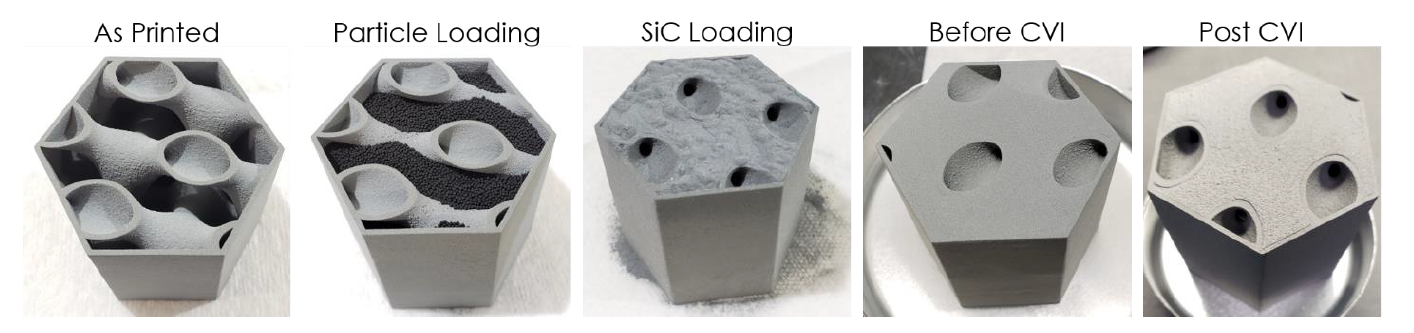
\includegraphics[width=\linewidth]{ornl-triso-print.png} 
    \caption{Stages of additive manufacturing fabrication conducted at \acrlong{ORNL} to 
    produce a fuel demonstration element with \gls{TRISO} particles embedded in 
    a SiC matrix \cite{trammell_advanced_2019}. Figure reproduced from 
    \cite{trammell_advanced_2019}.}
    \label{fig:ornl-triso-print}
\end{figure}
Figure \ref{fig:ornl-fuel-element} shows the fuel element manufactured at 
\gls{ORNL} for the \gls{TCR} program \cite{betzler_transformational_2020}. 
\begin{figure}[htb!]
    \centering
    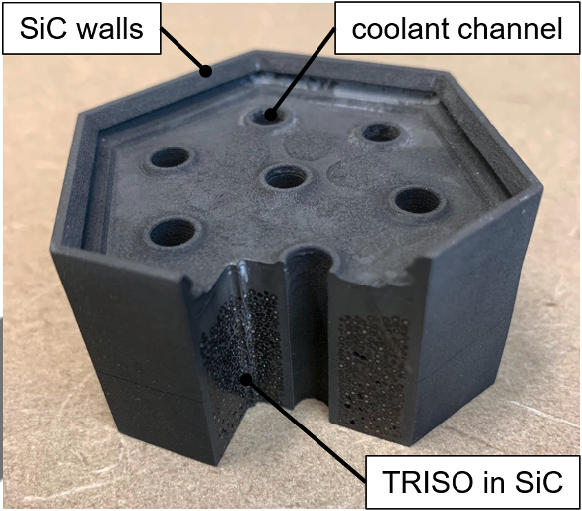
\includegraphics[width=0.6\linewidth]{ornl-fuel-element.png} 
    \caption{The top portion of the advanced manufactured fuel element 
    for the \acrfull{TCR} program at \acrfull{ORNL}.
    A cutaway of the element shows surrogate TRISO particles packed in the SiC matrix.
    Figure reproduced from \cite{betzler_transformational_2020}.}
    \label{fig:ornl-fuel-element}
\end{figure}
The current design uses axially uniform fuel shapes and coolant channels. 
The \gls{TCR} program plans to optimize the coolant channels to vary in axial 
and radial directions within the fuel element 
\cite{betzler_transformational_2020,sobes_artificial_2020}. 

Besides the \gls{TCR} program, the nuclear materials research community has made 
significant progress in demonstrating the application of additive manufacturing 
to nuclear fuel and structural core material fabrication. 
Rosales et al. \cite{rosales_characterizing_2019} conducted a feasibility study 
of direct routes to fabricate dense uranium silicide (U$_3$Si$_2$) fuel pellets 
using the \gls{INL} approach known as \gls{AMAFT}. 
U$_3$Si$_2$ demonstrates desirable accident-tolerant nuclear fuel properties 
such as high uranium density and improved thermal properties; however, it has 
an expensive and long metallurgical fabrication process. 
Thus, using \gls{AMAFT} to fabricate U$_3$Si$_2$ will lower costs and ensure a
timely and commercially-reliable fabrication process \cite{rosales_characterizing_2019}. 
Sridharan et al. \cite{sridharan_performance_2019} demonstrated applying
the laser-blown-powder additive manufacturing process to fabricate \gls{FM} steel, 
commonly used for cladding and structural components in nuclear reactors. 
Koyanagi et al. \cite{koyanagi_additive_2020} presented the latest 
additive manufacturing technology for manufacturing nuclear-grade \gls{SiC} materials. 
They demonstrated that combining additive manufacturing techniques and 
traditional \gls{SiC} densification methods enabled new designs of \gls{SiC} 
components with complex shapes. 
\gls{SiC} demonstrates excellent strength at elevated temperatures, chemical inertness, 
relatively low neutron absorption, and stability under neutron irradiation up 
to high doses \cite{sauder_ceramic_2014, snead_handbook_2007,koyanagi_additive_2020}. 
These qualities make \gls{SiC} suitable for many applications in nuclear systems, 
such as fuel cladding, constituents of fuel particles \cite{snead_handbook_2007} 
and pellets \cite{terrani_progress_2015}, and core structural components in fission 
reactors \cite{sauder_ceramic_2014}. 
% TODO: reichard and hosemann have also done work in this space with functionally 
% graded components. 

\section{Nuclear Reactor Design Optimization}
\label{sec:opt}
A nuclear reactor's complexity results in reactor design optimization being a 
multi-objective design problem requiring a tradeoff between desirable 
attributes \cite{byrne_evolving_2014,simon_sciences_2019}. 
When multiple conflicting objectives compete, no single optimum solution 
simultaneously optimizes all objectives. 
Instead, multi-objective optimization returns multiple optimal 
solutions that meet each objective to varying degrees; this set of solutions is 
the Pareto front \cite{deb_multi-objective_2001}. 
Figure \ref{fig:pareto} illustrates a two-dimensional problem's objective space and 
Pareto Front. 
\begin{figure}[htbp]
    \centering
    \includegraphics[width=0.7\linewidth]{example_pareto_front.png} 
    \caption{Illustration of an objective space and Pareto Front. Figure reproduced 
    from \cite{deb_multi-objective_2001}. 
    The f1 and f2 axes correspond to the optimization objectives.}
    \label{fig:pareto}
\end{figure}
For each solution in the Pareto front, none of the objective functions can be 
improved without degrading another objective.
An ideal optimization method for a multi-objective problem like reactor design 
should find widely spread solutions in the obtained Pareto front 
\cite{deb_multi-objective_2001}.  

Traditional manufacturing constraints result in most of the past nuclear reactor 
optimization work focusing on optimizing classical reactor 
parameters such as radius of fuel pellet and clad, enrichment of fuel, 
pin pitch, etc. 
The optimization methods used for reactor design optimization are either 
deterministic or stochastic. 
Deterministic optimization methods usually start from a guess solution.
Then, the algorithm suggests a search direction by applying local 
information to a pre-specified transition rule. 
Any better solution becomes the new solution, and the above procedure continues 
several times \cite{deb_multi-objective_2001}. 
Drawbacks of deterministic methods include: algorithms tend to get stuck at
suboptimal solutions, and an algorithm efficient in solving one type of problem 
may not solve a different problem efficiently \cite{deb_multi-objective_2001}. 
Stochastic optimization methods such as evolutionary algorithms and simulated annealing
minimize or maximize an objective function with randomness present. 
Stochasticity enables them to find globally optimal solutions more reliably than 
deterministic methods. 
Due to stochastic methods' many advantages, most efforts toward nuclear 
reactor optimization use these methods. 

Additive manufacturing advancements for reactor core components have
removed conventional reactor manufacturing geometric constraints such as slabs as fuel 
planks, cylinders as fuel rods, spheres as fuel pebbles, axis-aligned coolant 
channels, etc  \cite{sobes_artificial_2020}.
Reactor design objectives remain consistent with past objectives, such as 
minimizing fuel amount and minimizing the maximum fuel temperature for a given 
power level.
However, reactor designers can now approach nuclear design problems with truly 
arbitrary geometries and optimize beyond classical parameters to further enhance 
fuel performance and safety.
This has opened the door for a complete re-examination of reactor core 
optimization, determining the optimal arbitrary geometry 
and fuel distribution for a given objective function with a much smaller set of 
constraints \cite{sobes_artificial_2020}. 

I discuss the previous nuclear reactor optimization efforts for classical and 
arbitrary parameters in the subsequent sections.

\subsection{Reactor Optimization for Classical Parameters}
This section describes previous efforts towards reactor optimization for classical 
geometry parameters, such as radius of fuel pellet and clad, enrichment of fuel, 
pin pitch, etc. 
The most commonly used stochastic optimization methods for reactor design 
optimization are simulated annealing and evolutionary algorithms. 

\subsubsection{Reactor Optimization with Simulated Annealing Method}
Simulated annealing iteratively updates one candidate solution until it reaches 
the termination criteria. 
At each iteration, the simulated annealing algorithm selects a random move. 
If the selected move improves the solution, it is always accepted; however,  
if it does not improve the solution, the algorithm updates the solution with 
some probability of less than 1.

Sacco et al. \cite{sacco_two_2006,sacco_metropolis_2008} used stochastic 
simulated annealing and deterministic-stochastic hybrid optimization techniques 
to optimize reactor dimensions, enrichment, materials, etc., to 
minimize the average peaking factor in a three-enrichment-zone reactor. 
Odeh et al. \cite{odeh_core_2016} used the simulated annealing stochastic algorithm 
coupled with neutronics and thermal-hydraulics simulation tools, \gls{PARCS} and RELAP5
\cite{fletcher_relap5mod3_1992}, to develop an optimal \gls{NMR-50} core design 
with a 10-year cycle length and minimal fissile loading. 
Kropaczek et al. \cite{kropaczek_large-scale_2019} demonstrated the constraint 
annealing method: a highly scalable method based on the parallel simulated annealing 
method with mixing of states \cite{kropaczek_constraint_2019} to solve large-scale, 
multiconstrained \gls{LWR} fuel cycle optimization problems. 
These papers demonstrate the simulated annealing optimization method's success in 
reactor design optimization problems. 

Nuclear reactor optimization problems require computationally 
expensive neutronics and thermal-hydraulics software to compute the objective 
function and constraints. 
Multiple papers utilized stochastic optimization methods with surrogate models 
to reduce computational cost. 
The surrogate models reduce the computational cost by replacing high-fidelity
neutronics or thermal hydraulics simulations.
Betzler et al. \cite{betzler_design_2019} developed a systematic approach to 
build a surrogate model to serve in place of high-fidelity computational 
analyses. 
They leveraged the surrogate model with a simulated annealing optimization 
algorithm to generate optimized designs at a lower computational cost and
understand the impact of design decisions on desired metrics for \gls{HFIR} \gls{LEU} 
core designs.

The simulated annealing method uses a point-by-point approach:
one solution gets updated to a new solution in one iteration, which does not 
exploit parallel systems' advantages.
Finding an optimal solution with simulated annealing methods takes very long if 
high-fidelity computationally expensive codes compute the objective function and 
constraints.
Using a simulated annealing method is only practical with surrogate evaluation models, 
as described in Betzler et al. \cite{betzler_design_2019}.

\subsubsection{Reactor Optimization with Evolutionary Algorithm Method}
Contrary to a single solution per iteration in deterministic and stochastic 
simulated annealing methods, evolutionary algorithms use a population of 
solutions in each iteration \cite{deb_multi-objective_2001}. 
Evolutionary algorithm methods mimic nature's evolutionary principles by driving 
the search toward an optimal solution through population elimination and combinations. 

Peireira et al. \cite{pereira_coarse-grained_2003,pereira_parallel_2008} 
used a coarse-grained parallel genetic algorithm and a niching genetic algorithm
to minimize the average peaking factor in a three-enrichment-zone reactor. 
Kamalpour et al. \cite{kamalpour_smart_2020} utilized the imperialist competitive 
algorithm, an evolutionary algorithm, to optimize an \gls{FCM} fuelled 
\gls{PWR} to extend the reactor core cycle length. 
Kumar et al. \cite{kumar_new_2015} combined genetic algorithm optimization 
with a surrogate model to optimize for high breeding of $^{233}$U and $^{239}$Pu 
in desired power peaking limits and keff by varying: fuel pin 
radius,  fissile material isotopic enrichment, coolant mass flow rate, and 
core inlet coolant temperature.

With the affordability and availability of parallel computing systems, the 
evolutionary algorithm optimization method stands out as a method 
that easily and conveniently exploits parallel systems. 
Further, evolutionary algorithms have proved amenable to \gls{HPC} solutions and 
scalable to tens of thousands of processors \cite{kropaczek_constraint_2019}. 
Thus, for optimization problems that require high-fidelity evaluation software, 
the evolutionary algorithm method can leverage parallel computing to find a 
solution faster than the simulated annealing method.
Therefore, I will utilize the evolutionary algorithm optimization method in 
this dissertation.
Section \ref{sec:ea} provides an overview of the literature on evolutionary algorithms.

\subsection{Reactor Optimization for Arbitrary Parameters}
\label{sec:lit-review-reactor-arbitrary}
Additive manufacturing advancements for reactor core components have
removed conventional reactor manufacturing geometric constraints such as slabs as fuel 
planks, cylinders as fuel rods, spheres as fuel pebbles, axis-aligned coolant 
channels, etc \cite{sobes_artificial_2020}.
Reactor designers can now approach nuclear design problems with truly 
arbitrary geometries and optimize beyond classical parameters to further enhance 
fuel performance and safety.
This section describes previous efforts towards reactor optimization for arbitrary 
geometry parameters. 

Sobes et al. \cite{sobes_artificial_2020} used a genetic algorithm to find 
minimum volume geometric configurations for a \gls{TCR}-like reactor with 
multiphysics constraints of 1500 pcm excess reactivity and maximum fuel 
temperature of 618 $^{\circ}C$ under forced-flow cooling conditions. 
This study represented arbitrary geometry variations using right cylinders.
The authors acknowledge that this work is only a first step towards truly 
arbitrary geometry expression. 
They found that the optimal cone-like core configuration has a truncated annular 
cone geometry, with the inlet surface being larger than the outlet 
\cite{sobes_artificial_2020}.

See et al. \cite{see_design_2022} conducted design optimization of the 
\gls{TCR}'s outlet plenum design with a Siemens design optimization tool, HEEDS,
and the \gls{CFD} code, STAR-CCM+. 
They had to design an instrumentation plane to monitor core coolant flow average 
temperature within $\pm 5 ^{\circ}C$ while maintaining a tight design 
constraint of 0.5-psi pressure drop across the outlet plenum.
The optimal design maintained a pressure drop to 0.49 psi with an instrumentation 
plane temperature standard deviation of $1.03^{\circ}C$. 
Figure \ref{fig:compare-outlet-plenum} shows the initial and optimal outlet plenum 
designs. 
Figure \ref{fig:see3} demonstrates how the optimal design impacted the stream 
tubes and enabled a smaller temperature standard deviation in the 
instrumentation plane. 
\begin{figure}[htb!]
    \centering
    \begin{subfigure}{0.49\textwidth}
        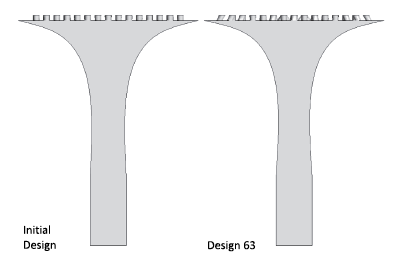
\includegraphics[width=\linewidth]{see1.png}
        \caption{Geometric representation of outer wall spline.}
        \label{fig:see1} 
    \end{subfigure}
    \begin{subfigure}{0.49\textwidth}
        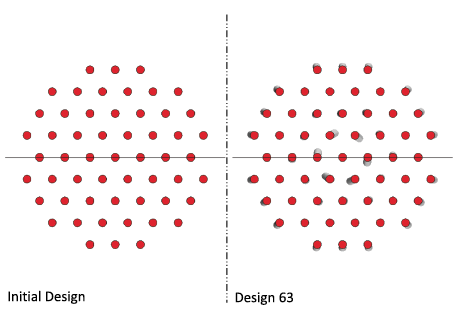
\includegraphics[width=\linewidth]{see2.png}
        \caption{Geometric representation of inlet channels.}
        \label{fig:see2} 
    \end{subfigure}
    \caption{Initial design versus the optimal design of outlet plenum from the study 
    by See et al. 
    The optimal design meets the following design objectives: 0.5-psi pressure drop 
    across the outlet plenum, monitor core coolant flow average temperature within 
    $\pm 5 ^{\circ}C$.
    Figures reproduced from \cite{betzler_transformational_2020}.}
    \label{fig:compare-outlet-plenum}
\end{figure}
\begin{figure}[htb!]
    \centering
    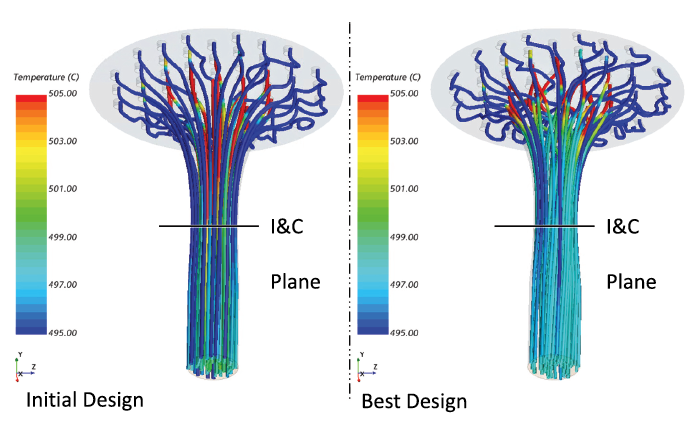
\includegraphics[width=0.9\linewidth]{see3.png} 
    \caption{Initial design versus optimal design of stream tubes in the outlet 
    plenum from the study by See et al. 
    The optimal design meets the following design objectives: 0.5-psi pressure 
    drop across the outlet plenum, monitor core coolant flow average temperature 
    within $\pm 5 ^{\circ}C$.
    Figures reproduced from \cite{see_design_2022}.}
    \label{fig:see3}
\end{figure}

Reactor optimization for arbitrary parameters is a new concept within the reactor 
optimization field, and only a few research demonstrations have begun exploring the 
large new design space.
Other fields that require 3D design optimization, such as architecture and mechanical 
design, are further along than the nuclear reactor optimization industry 
and have coined this type of optimization as generative design 
\cite{meintjes_generative_nodate}. 
As additive manufacturing technology advances and the \gls{TCR} program 
demonstrates the first 3D printed operational reactor, more reactor designers 
will begin to explore the huge design space enabled by 3D printing. 
Thoroughly exploring the design space using additive manufacturing should allow 
the placement of fuel, moderation, and coolant material in any possible location, 
within physical limits. 
In this dissertation, I will begin to explore the large design space while 
also acknowledging (like the authors in \cite{sobes_artificial_2020}) that 
this work is only an intermediate step towards developing a truly arbitrary 
geometry expression. 

\section{Evolutionary Algorithms} 
\label{sec:ea}
The expanded design space associated with an arbitrary reactor geometry increases 
the time required for reactor designers to thoroughly explore and find optimal 
geometries.
Instead, reactor designers can leverage \gls{AI} optimization methods, such as 
evolutionary algorithms, to rapidly explore the large design space to find global 
optimal designs. 
\gls{AI} does not replace the human reactor designer, but shifts the human 
designer's focus away from conjecturing suitable geometries to defining design 
criteria to find optimal designs \cite{sobes_artificial_2020}. 
Thus, when the human designer changes the reactor criteria, the \gls{AI} 
model will quickly adapt and produce new global optimal designs to fit the new 
criteria.  
This optimization method is also known as generative design. 
In this dissertation, I utilize the evolutionary algorithm optimization method 
for generative reactor design as evolutionary algorithms have proven to find globally 
optimal solutions robustly and can take advantage of parallel systems. 

Evolutionary algorithms create a population of individual solutions inspired 
by biological evolution and induce goals by using a `fitness function' to 
mutate and preferentially replicate high-scoring individuals to reach an 
optimal solution.
Evolutionary algorithms often perform well at approximating solutions to many 
problem types because they do not make assumptions about the 
underlying fitness landscape.
Genetic algorithms are the most popular evolutionary algorithms for solving 
multi-objective problems \cite{byrne_evolving_2014, krish_practical_2011}. 
In this dissertation, I use the terms evolutionary and genetic algorithms 
interchangeably to refer to genetic algorithms.

\subsection{Genetic Algorithms}
\label{sec:genetic_alg}
Genetic algorithms imitate natural genetics and selection to evolve solutions 
by maintaining a population of solutions, allowing fitter solutions to reproduce,
and letting less fit solutions die off, resulting in final solutions that are 
better than the previous generations \cite{renner_genetic_2003}. 
I will refer to a solution as an individual within the population. 
Genetic algorithms efficiently exploit historical information to speculate new
 search points, improving each subsequent population's performance 
\cite{goldberg_genetic_1989}. 
They are theoretically and empirically proven to provide robust 
search in complex spaces and are computationally simple yet powerful 
in their search for improvement \cite{goldberg_genetic_1989}. 
Genetic algorithms trounce deterministic and stochastic simulated 
annealing optimization methods because they:
\begin{enumerate}
    \item search from a population of points
    \item use objective function information, not derivatives or other 
    auxiliary knowledge of the problem
    \item use probabilistic transition rules, not deterministic rules
\end{enumerate}
Figure \ref{fig:genetic_alg} depicts the iterative process of using a genetic algorithm
to solve a problem. 
The genetic algorithm generates new populations iteratively until it meets the termination 
criteria. 
\begin{figure}[htb!]
        \centering
        \begin{tikzpicture}[node distance=1.7cm]
                \tikzstyle{every node}=[font=\small]
                \node (1) [lbblock] {\textbf{Create initial population}};
                \node (2) [lbblock, below of=1] {\textbf{Evaluate initial population}};
                \node (3) [lbblock, below of=2, yshift = -1.3cm] {\textbf{Create new population:} \\ 
                \begin{enumerate} \item \textbf{Select} individuals for mating 
                                  \item Create offspring by \textbf{crossover} 
                                  \item \textbf{Mutate} selected individuals 
                                  \item Keep selected individuals from previous generation
                                 \end{enumerate}};
                \node (4) [lbblock, below of=3, yshift=-1.3cm] {\textbf{Evaluate new population}};
                \node (5) [lbblock, below of=4] {\textbf{Is termination \\ criteria satisfied?}};
                \node (6) [lbblock, below of=5] {\textbf{Best solution is returned!}};
                \draw [arrow] (1) -- (2);
                \draw [arrow] (2) -- (3);
                \draw [arrow] (3) -- (4);
                \draw [arrow] (4) -- (5);
                \draw [arrow] (5) -- node[anchor=east] {yes} (6);
                \draw [arrow] (5) -- ([shift={(0.5cm,0cm)}]5.east)-- node[anchor=west] {no} ([shift={(0.5cm,0cm)}]3.east)--(3);
        \end{tikzpicture}
        \caption{Process of finding optimal solutions for a problem with a 
        evolutionary algorithm \cite{renner_genetic_2003}. }
        \label{fig:genetic_alg}
\end{figure}

Genetic algorithms use mechanisms inspired by biological evolution, such as 
selection, crossover, and mutation. 
The three operators are simple and straightforward.
The crossover operator recombines good individuals to form a better 
individual. 
The mutation operator alters individuals to create better individuals
\cite{deb_multi-objective_2001}.  
The selection operator selects good individuals. 
The selection operator does not create new individuals in the population 
and only makes more copies of good individuals at the expense of not-so-good
individuals. 
The crossover and mutation operators perform the creation of new solutions.
Next, we provide more descriptions and common methods for each operator.

\subsubsection{Crossover/Mating Operator}
In most crossover operators, the operator randomly picks two individuals from 
the population. 
The operator exchanges some portion of each individuals' attributes with one 
another to create two new individuals \cite{deb_multi-objective_2001}. 
Crossover operator methods utilized in this dissertation include 
\textit{single-point crossover}, \textit{uniform crossover}, and 
\textit{blend crossover}. 
In the \textit{single-point crossover}, the operator randomly selects two 
individuals from the population and a site along the individual's definition. 
For example, if the individual is a list, the operator randomly chooses an element 
in the list as the cross-site. 
Then, the attributes on the cross site's right side are exchanged between the two 
individuals, creating two new offspring individuals. 
In a \textit{uniform crossover}, the user defines an independent exchange probability 
for each individual's attribute.
In \textit{blend crossover}, the operator creates two offspring (O) individuals based on 
a linear combination of two-parent (P) individuals using the following equations: 
\begin{align}
    O_1 &= P_1 - \alpha(P_1-P_2) \\
    O_2 &= P_2 + \alpha(P_1-P_2)
\intertext{where}
\alpha &= \mbox{Extent of the interval in which the new values can be drawn} \nonumber \\
 & \mbox{for each attribute on both side of the parents’ attributes (user-defined)} \nonumber 
\end{align}

The user defines a crossover probability ($p_c$) to preserve some good 
individuals selected during the selection operator stage.  
Therefore, the crossover operator only operates on $100p_c\%$ of the 
population; the rest proceed to the new population \cite{deb_multi-objective_2001}. 
The crossover operator covers the search aspect of the genetic algorithms, 
whereas the mutation operator keeps diversity in the population 
\cite{deb_multi-objective_2001}. 

\subsubsection{Mutation Operator}
The mutation operator alters one or more attributes of an individual within 
a population. 
Mutation operator methods utilized in this dissertation include 
\textit{polynomial bounded mutation}, in which each attribute in each individual 
is mutated based on a polynomial distribution. 
The user also defines each attribute's upper and lower bounds and the 
crowding degree of the mutation, $\eta$ (a big $\eta$ will produce a mutant 
resembling its parent, while a small $\eta$ will produce the opposite).
Mutation occurs in the genetic algorithm based on a user-defined mutation 
probability ($p_m$). 
A low $p_m$ prevents a primitive random search. 

\subsubsection{Selection Operator}
% this section needs improvement. 
The selection operator duplicates good individuals and eliminates bad individuals 
while keeping the population constant \cite{deb_multi-objective_2001}. 
It achieves this by identifying above-average individuals, eliminating bad 
individuals from the population, and replacing them with copies of good individuals.
Selection operator methods utilized in this dissertation include \textit{tournament 
selection}, \textit{best selection}, and \textit{\gls{NSGA-II} selection}. 
In \textit{tournament selection}, a user-defined number of individuals play in a
tournament, and the best individual proceeds to the next population. 
The tournament repeats until all the population's spots are filled.
In \textit{best selection}, the operator selects a user-defined number of best 
individuals, and copies are made to keep the population size constant. 
In \textit{NSGA-II selection}, the elitist operator selects the best individuals 
from the combination of parent and offspring populations \cite{deb_fast_2002}.
\textit{NSGA-II selection} works well for multi-objective optimization. 

\subsection{Genetic Algorithm Hyperparameter Tuning}
\label{sec:balance}
Hyperparameters refer to parameters whose value controls 
the genetic algorithm's process, such as the population size. 
A well-performing genetic algorithm needs to balance the extent of exploration and 
exploitation; by finding a balance between the conservation of 
valuable individuals obtained until the current generation while exploring new 
individuals. 
With overexploitation of previously obtained individuals, the population loses 
diversity, resulting in premature convergence to a suboptimal solution. 
Alternatively, with over-exploration, the algorithm does not appropriately utilize 
the information obtained thus far, and the genetic algorithm's search procedure 
behaves like a random search process
\cite{deb_multi-objective_2001}. 

A quantitative balance between these two issues, exploitation and exploration, 
is challenging to achieve. 
Deb et al. \cite{deb_multi-objective_2001} and Goldberg et al. 
\cite{goldberg_toward_1993} quantified the relationship between exploitation 
and exploration. 
They found that for the one-max test problem, in which the objective seeks to 
maximize the number of 1s in a string, a genetic algorithm with any arbitrary 
hyperparameter setting does not work well even on a simple problem. 
Only genetic algorithms with a selection pressure (s) and crossover probability ($p_c$) 
falling inside the control map (Figure \ref{fig:controlmap}) will find the desired 
optimum.  
\begin{figure}[htb!]
    \centering
    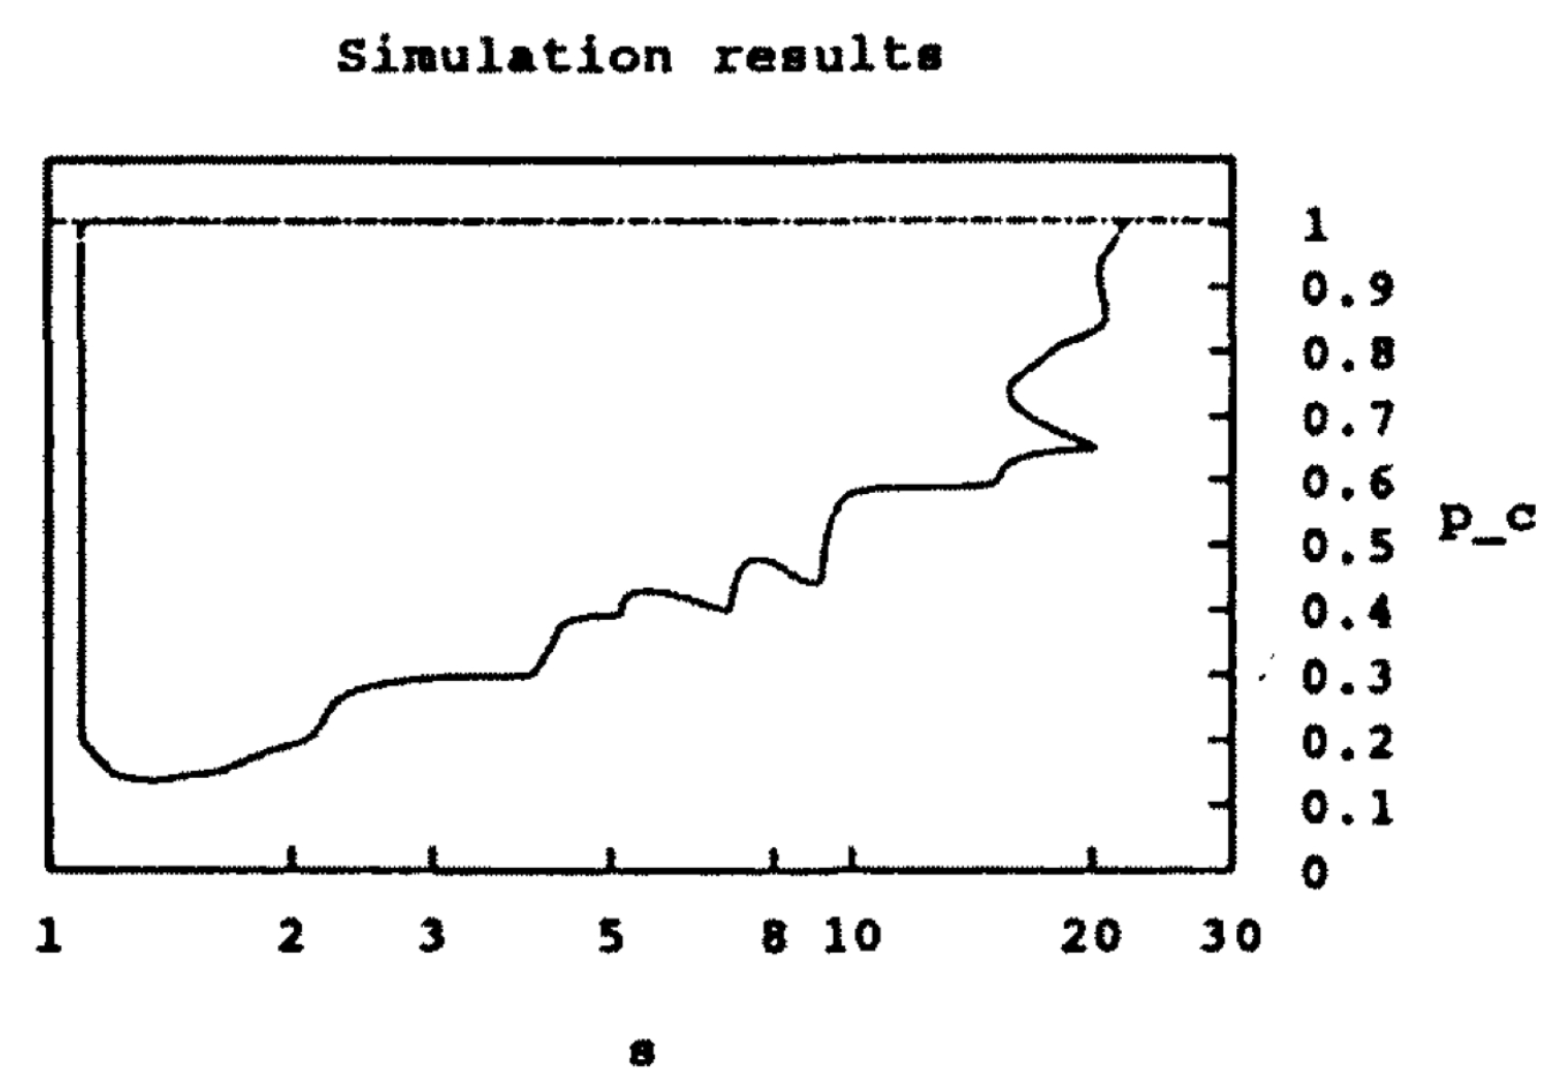
\includegraphics[width=0.6\linewidth]{controlmap.png} 
    \caption{Control map region of selection pressure (s) and crossover probability 
    ($p_c$) values in which the genetic algorithm will find the desired optimum for the 
    one-max problem.
    Figure reproduced from \cite{goldberg_toward_1993,deb_multi-objective_2001}.}
    \label{fig:controlmap}
\end{figure}
Another consideration is the population size. 
A function with considerable variability in objective function values demands 
a large population size to find a global optimum \cite{deb_multi-objective_2001}. 
Therefore, finding an optimized solution with genetic algorithms requires the user 
to conduct a hyperparameter search. 

Ng et al. \cite{ng_improving_2021} suggest that a coarse-to-fine sampling scheme 
is the best way to perform a systematic hyperparameter search.  
For a two-dimensional example of a coarse-to-fine sampling scheme, the user 
first does a coarse sample of the entire square, then a fine search on the 
coarse search's best-performing region. 
Ng et al. also suggest using random sampling over grid sampling because of the 
former's efficiency in high-dimensional spaces. 
Figure \ref{fig:random_vs_grid_sampling} illustrates how grid sampling gives 
even coverage in the original 2-d space but provides inefficient coverage in 
projections onto either the x1 or x2 subspace.  
In contrast, random sampling produces a less even distribution in the original 
space but a far more even distribution in the subspaces.
\begin{figure}[htb!]
    \centering
    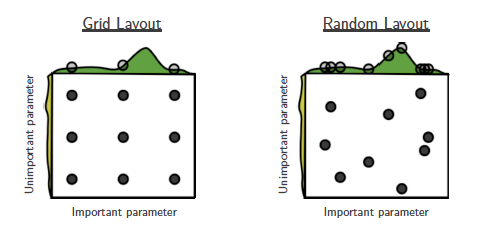
\includegraphics[width=0.8\linewidth]{random_vs_grid_sampling.png} 
    \caption{The impact of grid sampling vs random sampling on coverage of projections 
    into subspaces (reproduced from \cite{jordan_hyperparameter_2017}). 
    Random sampling has better coverage in the subspaces.}
    \label{fig:random_vs_grid_sampling}
\end{figure}

\section{Summary}
This chapter provided a literature review of relevant past research efforts that 
give context to and sipport the work of this dissertation. 
In summary, participation in the \acrfull{OECD}-\acrfull{NEA} \acrfull{FHR} 
benchmarking exercise contributes to assessing the current neutron transport and 
thermal-hydraulics modeling and simulation capabilities for the \acrfull{AHTR} design.
Furthermore, additive manufacturing of nuclear reactor components is a quickly 
developing field due to advancements driven by the aerospace and automotive industries, 
which led to breakthroughs in metal component additive manufacturing fabrication. 
The promise of cheaper and faster manufacturing of reactor components with 
additive manufacturing frees complex reactor geometries from previous 
manufacturing constraints and allows reactor designers to reexamine reactor 
design optimization.  
Stochastic optimization methods such as evolutionary algorithms have proven to 
work well for finding global optimums in multi-objective design problems such as 
nuclear reactor optimization and can be leveraged to explore the vast exploration 
design space enabled by additive manufacturing.
